% Options for packages loaded elsewhere
\PassOptionsToPackage{unicode}{hyperref}
\PassOptionsToPackage{hyphens}{url}
%
\documentclass[
  8pt,
  ignorenonframetext,
]{beamer}
\author{}
\date{\vspace{-2.5em}}

\usepackage{pgfpages}
\setbeamertemplate{caption}[numbered]
\setbeamertemplate{caption label separator}{: }
\setbeamercolor{caption name}{fg=normal text.fg}
\beamertemplatenavigationsymbolsempty
% Prevent slide breaks in the middle of a paragraph
\widowpenalties 1 10000
\raggedbottom
\setbeamertemplate{part page}{
  \centering
  \begin{beamercolorbox}[sep=16pt,center]{part title}
    \usebeamerfont{part title}\insertpart\par
  \end{beamercolorbox}
}
\setbeamertemplate{section page}{
  \centering
  \begin{beamercolorbox}[sep=12pt,center]{part title}
    \usebeamerfont{section title}\insertsection\par
  \end{beamercolorbox}
}
\setbeamertemplate{subsection page}{
  \centering
  \begin{beamercolorbox}[sep=8pt,center]{part title}
    \usebeamerfont{subsection title}\insertsubsection\par
  \end{beamercolorbox}
}
\AtBeginPart{
  \frame{\partpage}
}
\AtBeginSection{
  \ifbibliography
  \else
    \frame{\sectionpage}
  \fi
}
\AtBeginSubsection{
  \frame{\subsectionpage}
}
\usepackage{amsmath,amssymb}
\usepackage{lmodern}
\usepackage{iftex}
\ifPDFTeX
  \usepackage[T1]{fontenc}
  \usepackage[utf8]{inputenc}
  \usepackage{textcomp} % provide euro and other symbols
\else % if luatex or xetex
  \usepackage{unicode-math}
  \defaultfontfeatures{Scale=MatchLowercase}
  \defaultfontfeatures[\rmfamily]{Ligatures=TeX,Scale=1}
\fi
% Use upquote if available, for straight quotes in verbatim environments
\IfFileExists{upquote.sty}{\usepackage{upquote}}{}
\IfFileExists{microtype.sty}{% use microtype if available
  \usepackage[]{microtype}
  \UseMicrotypeSet[protrusion]{basicmath} % disable protrusion for tt fonts
}{}
\makeatletter
\@ifundefined{KOMAClassName}{% if non-KOMA class
  \IfFileExists{parskip.sty}{%
    \usepackage{parskip}
  }{% else
    \setlength{\parindent}{0pt}
    \setlength{\parskip}{6pt plus 2pt minus 1pt}}
}{% if KOMA class
  \KOMAoptions{parskip=half}}
\makeatother
\usepackage{xcolor}
\IfFileExists{xurl.sty}{\usepackage{xurl}}{} % add URL line breaks if available
\IfFileExists{bookmark.sty}{\usepackage{bookmark}}{\usepackage{hyperref}}
\hypersetup{
  hidelinks,
  pdfcreator={LaTeX via pandoc}}
\urlstyle{same} % disable monospaced font for URLs
\newif\ifbibliography
\usepackage{color}
\usepackage{fancyvrb}
\newcommand{\VerbBar}{|}
\newcommand{\VERB}{\Verb[commandchars=\\\{\}]}
\DefineVerbatimEnvironment{Highlighting}{Verbatim}{commandchars=\\\{\}}
% Add ',fontsize=\small' for more characters per line
\usepackage{framed}
\definecolor{shadecolor}{RGB}{248,248,248}
\newenvironment{Shaded}{\begin{snugshade}}{\end{snugshade}}
\newcommand{\AlertTok}[1]{\textcolor[rgb]{0.94,0.16,0.16}{#1}}
\newcommand{\AnnotationTok}[1]{\textcolor[rgb]{0.56,0.35,0.01}{\textbf{\textit{#1}}}}
\newcommand{\AttributeTok}[1]{\textcolor[rgb]{0.77,0.63,0.00}{#1}}
\newcommand{\BaseNTok}[1]{\textcolor[rgb]{0.00,0.00,0.81}{#1}}
\newcommand{\BuiltInTok}[1]{#1}
\newcommand{\CharTok}[1]{\textcolor[rgb]{0.31,0.60,0.02}{#1}}
\newcommand{\CommentTok}[1]{\textcolor[rgb]{0.56,0.35,0.01}{\textit{#1}}}
\newcommand{\CommentVarTok}[1]{\textcolor[rgb]{0.56,0.35,0.01}{\textbf{\textit{#1}}}}
\newcommand{\ConstantTok}[1]{\textcolor[rgb]{0.00,0.00,0.00}{#1}}
\newcommand{\ControlFlowTok}[1]{\textcolor[rgb]{0.13,0.29,0.53}{\textbf{#1}}}
\newcommand{\DataTypeTok}[1]{\textcolor[rgb]{0.13,0.29,0.53}{#1}}
\newcommand{\DecValTok}[1]{\textcolor[rgb]{0.00,0.00,0.81}{#1}}
\newcommand{\DocumentationTok}[1]{\textcolor[rgb]{0.56,0.35,0.01}{\textbf{\textit{#1}}}}
\newcommand{\ErrorTok}[1]{\textcolor[rgb]{0.64,0.00,0.00}{\textbf{#1}}}
\newcommand{\ExtensionTok}[1]{#1}
\newcommand{\FloatTok}[1]{\textcolor[rgb]{0.00,0.00,0.81}{#1}}
\newcommand{\FunctionTok}[1]{\textcolor[rgb]{0.00,0.00,0.00}{#1}}
\newcommand{\ImportTok}[1]{#1}
\newcommand{\InformationTok}[1]{\textcolor[rgb]{0.56,0.35,0.01}{\textbf{\textit{#1}}}}
\newcommand{\KeywordTok}[1]{\textcolor[rgb]{0.13,0.29,0.53}{\textbf{#1}}}
\newcommand{\NormalTok}[1]{#1}
\newcommand{\OperatorTok}[1]{\textcolor[rgb]{0.81,0.36,0.00}{\textbf{#1}}}
\newcommand{\OtherTok}[1]{\textcolor[rgb]{0.56,0.35,0.01}{#1}}
\newcommand{\PreprocessorTok}[1]{\textcolor[rgb]{0.56,0.35,0.01}{\textit{#1}}}
\newcommand{\RegionMarkerTok}[1]{#1}
\newcommand{\SpecialCharTok}[1]{\textcolor[rgb]{0.00,0.00,0.00}{#1}}
\newcommand{\SpecialStringTok}[1]{\textcolor[rgb]{0.31,0.60,0.02}{#1}}
\newcommand{\StringTok}[1]{\textcolor[rgb]{0.31,0.60,0.02}{#1}}
\newcommand{\VariableTok}[1]{\textcolor[rgb]{0.00,0.00,0.00}{#1}}
\newcommand{\VerbatimStringTok}[1]{\textcolor[rgb]{0.31,0.60,0.02}{#1}}
\newcommand{\WarningTok}[1]{\textcolor[rgb]{0.56,0.35,0.01}{\textbf{\textit{#1}}}}
\setlength{\emergencystretch}{3em} % prevent overfull lines
\providecommand{\tightlist}{%
  \setlength{\itemsep}{0pt}\setlength{\parskip}{0pt}}
\setcounter{secnumdepth}{-\maxdimen} % remove section numbering
% type setting
% ------------------------------------------------------------------------------
\usepackage[german]{babel}     

% fonts
% ------------------------------------------------------------------------------
\usefonttheme{professionalfonts}

% slide title and horizontal line
% ------------------------------------------------------------------------------
\setbeamertemplate{frametitle}{%
    \vskip-30pt \color{black}\large%
    \begin{minipage}[b][23pt]{120mm}%
    \flushleft\insertframetitle%
    \end{minipage}%
}

\setbeamertemplate{headline}										
{
\vskip10pt\hfill\hspace{3.5mm} 										 
\vskip15pt\color{black}\rule{\textwidth}{0.4pt} 					 
}

% slide number
% ---------------------------------------------------------------
\setbeamertemplate{navigation symbols}{}
\setbeamertemplate{footline}
{
\vskip5pt
\vskip2pt
\makebox[123mm]{\hspace{7.5mm}
\hfill Allgemeines Lineares Modell $\vert$ 
\copyright $ $ 2022 Dirk Ostwald CC BY-NC-SA 4.0 $\vert$ 
Folie \insertframenumber}
\vskip4pt
}

% block color scheme
% ------------------------------------------------------------------------------
% colors
\definecolor{white}{RGB}{255,255,255}
\definecolor{grey}{RGB}{235,235,235}
\definecolor{lightgrey}{RGB}{245,245,245}
\definecolor{LightBlue}{RGB}{220,220,255}
\definecolor{darkblue}{RGB}{51, 51, 153}

% definitions and theorems
\setbeamercolor{block title}{fg = black, bg = grey}
\setbeamercolor{block body}{fg = black, bg = lightgrey}

% general line spacing 
% ------------------------------------------------------------------------------
\linespread{1.3}

% local line spacing
% ------------------------------------------------------------------------------
\usepackage{setspace}

% colors
% -----------------------------------------------------------------------------
\usepackage{color}

% justified text
% ------------------------------------------------------------------------------
\usepackage{ragged2e}
\usepackage{etoolbox}
\apptocmd{\frame}{}{\justifying}{}

% bullet point lists
% -----------------------------------------------------------------------------
\setbeamertemplate{itemize item}[circle]
\setbeamertemplate{itemize subitem}[circle]
\setbeamertemplate{itemize subsubitem}[circle]
\setbeamercolor{itemize item}{fg = black}
\setbeamercolor{itemize subitem}{fg = black}
\setbeamercolor{itemize subsubitem}{fg = black}
\setbeamercolor{enumerate item}{fg = black}
\setbeamercolor{enumerate subitem}{fg = black}
\setbeamercolor{enumerate subsubitem}{fg = black}
\setbeamerfont{itemize/enumerate body}{}
\setbeamerfont{itemize/enumerate subbody}{size = \normalsize}
\setbeamerfont{itemize/enumerate subsubbody}{size = \normalsize}

% color links
% ------------------------------------------------------------------------------
\usepackage{hyperref}
\definecolor{urls}{RGB}{204,0,0}
\hypersetup{colorlinks, citecolor = darkblue, urlcolor = urls}


% additional math commands
% ------------------------------------------------------------------------------
\usepackage{bm}                                         
\newcommand{\niton}{\not\owns}
\DeclareMathOperator*{\intinf}{\int_{-\infty}^{\infty}}


% text highlighting
% ------------------------------------------------------------------------------
\usepackage{soul}
\makeatletter
\let\HL\hl
\renewcommand\hl{%
  \let\set@color\beamerorig@set@color
  \let\reset@color\beamerorig@reset@color
  \HL}
\makeatother

% equation highlighting
% -----------------------------------------------------------------------------
\newcommand{\highlight}[2][yellow]{\mathchoice%
  {\colorbox{#1}{$\displaystyle#2$}}%
  {\colorbox{#1}{$\textstyle#2$}}%
  {\colorbox{#1}{$\scriptstyle#2$}}%
  {\colorbox{#1}{$\scriptscriptstyle#2$}}}%

% additional mathematical operators
% ------------------------------------------------------------------------------
\DeclareMathOperator*{\argmax}{arg\,max}
\DeclareMathOperator*{\argmin}{arg\,min}

\ifLuaTeX
  \usepackage{selnolig}  % disable illegal ligatures
\fi

\begin{document}

\begin{frame}[plain]{}
\protect\hypertarget{section}{}
\center

\begin{center}
\includegraphics[width=0.2\linewidth]{5_Abbildungen/alm_5_otto} \end{center}

\vspace{2mm}

\huge

Allgemeines Lineares Modell \vspace{6mm}

\large

BSc Psychologie SoSe 2022

\vspace{6mm}
\normalsize

Prof.~Dr.~Dirk Ostwald
\end{frame}

\begin{frame}[plain]{}
\protect\hypertarget{section-1}{}
\center
\huge
\vfill

\noindent (5) Modellformulierung \vfill
\end{frame}

\begin{frame}{Überblick}
\protect\hypertarget{uxfcberblick}{}
\small
\center
\footnotesize
\renewcommand{\arraystretch}{1.1}
\begin{tabular}{lll}
Datum        & Einheit                       & Thema                                              \\\hline
08.04.2022   & Grundlagen                    & (1) Regression                                 \\
             & \textcolor{gray}{Osterpause}                                             \\
22.04.2022   & Grundlagen                    & (2) Korrelation                            \\
29.04.2022   & Grundlagen                    & (3) Matrizen                             \\
06.05.2022   & Grundlagen                    & (4) Normalverteilungen                   \\
13.05.2022   & Theorie                       & (5) Modellformulierung                   \\
20.05.2022   & Theorie                       & (6) Modellschätzung                      \\
27.05.2022   & Theorie                       & (7) Modellevaluation                     \\
03.06.2021   & Anwendung                     & (8) Studiendesign                        \\
10.06.2021   & Anwendung                     & (9) T-Tests                              \\
17.06.2021   & Anwendung                     & (10) Einfaktorielle Varianzanalyse       \\
24.06.2022   & Anwendung                     & (11) Zweifaktorielle Varianzanalyse      \\
01.07.2022   & Anwendung                     & (12) Multiple Regression                 \\
08.07.2022   & Anwendung                     & (13) Kovarianzanalyse                    \\\hline
Juli 2022    & Klausurtermin                 &                                          \\
März 2023    & Klausurwiederholungstermin    &
\end{tabular}
\end{frame}

\begin{frame}{Überblick}
\protect\hypertarget{uxfcberblick-1}{}
\large

Naturwissenschaft \vspace{7mm}

\begin{center}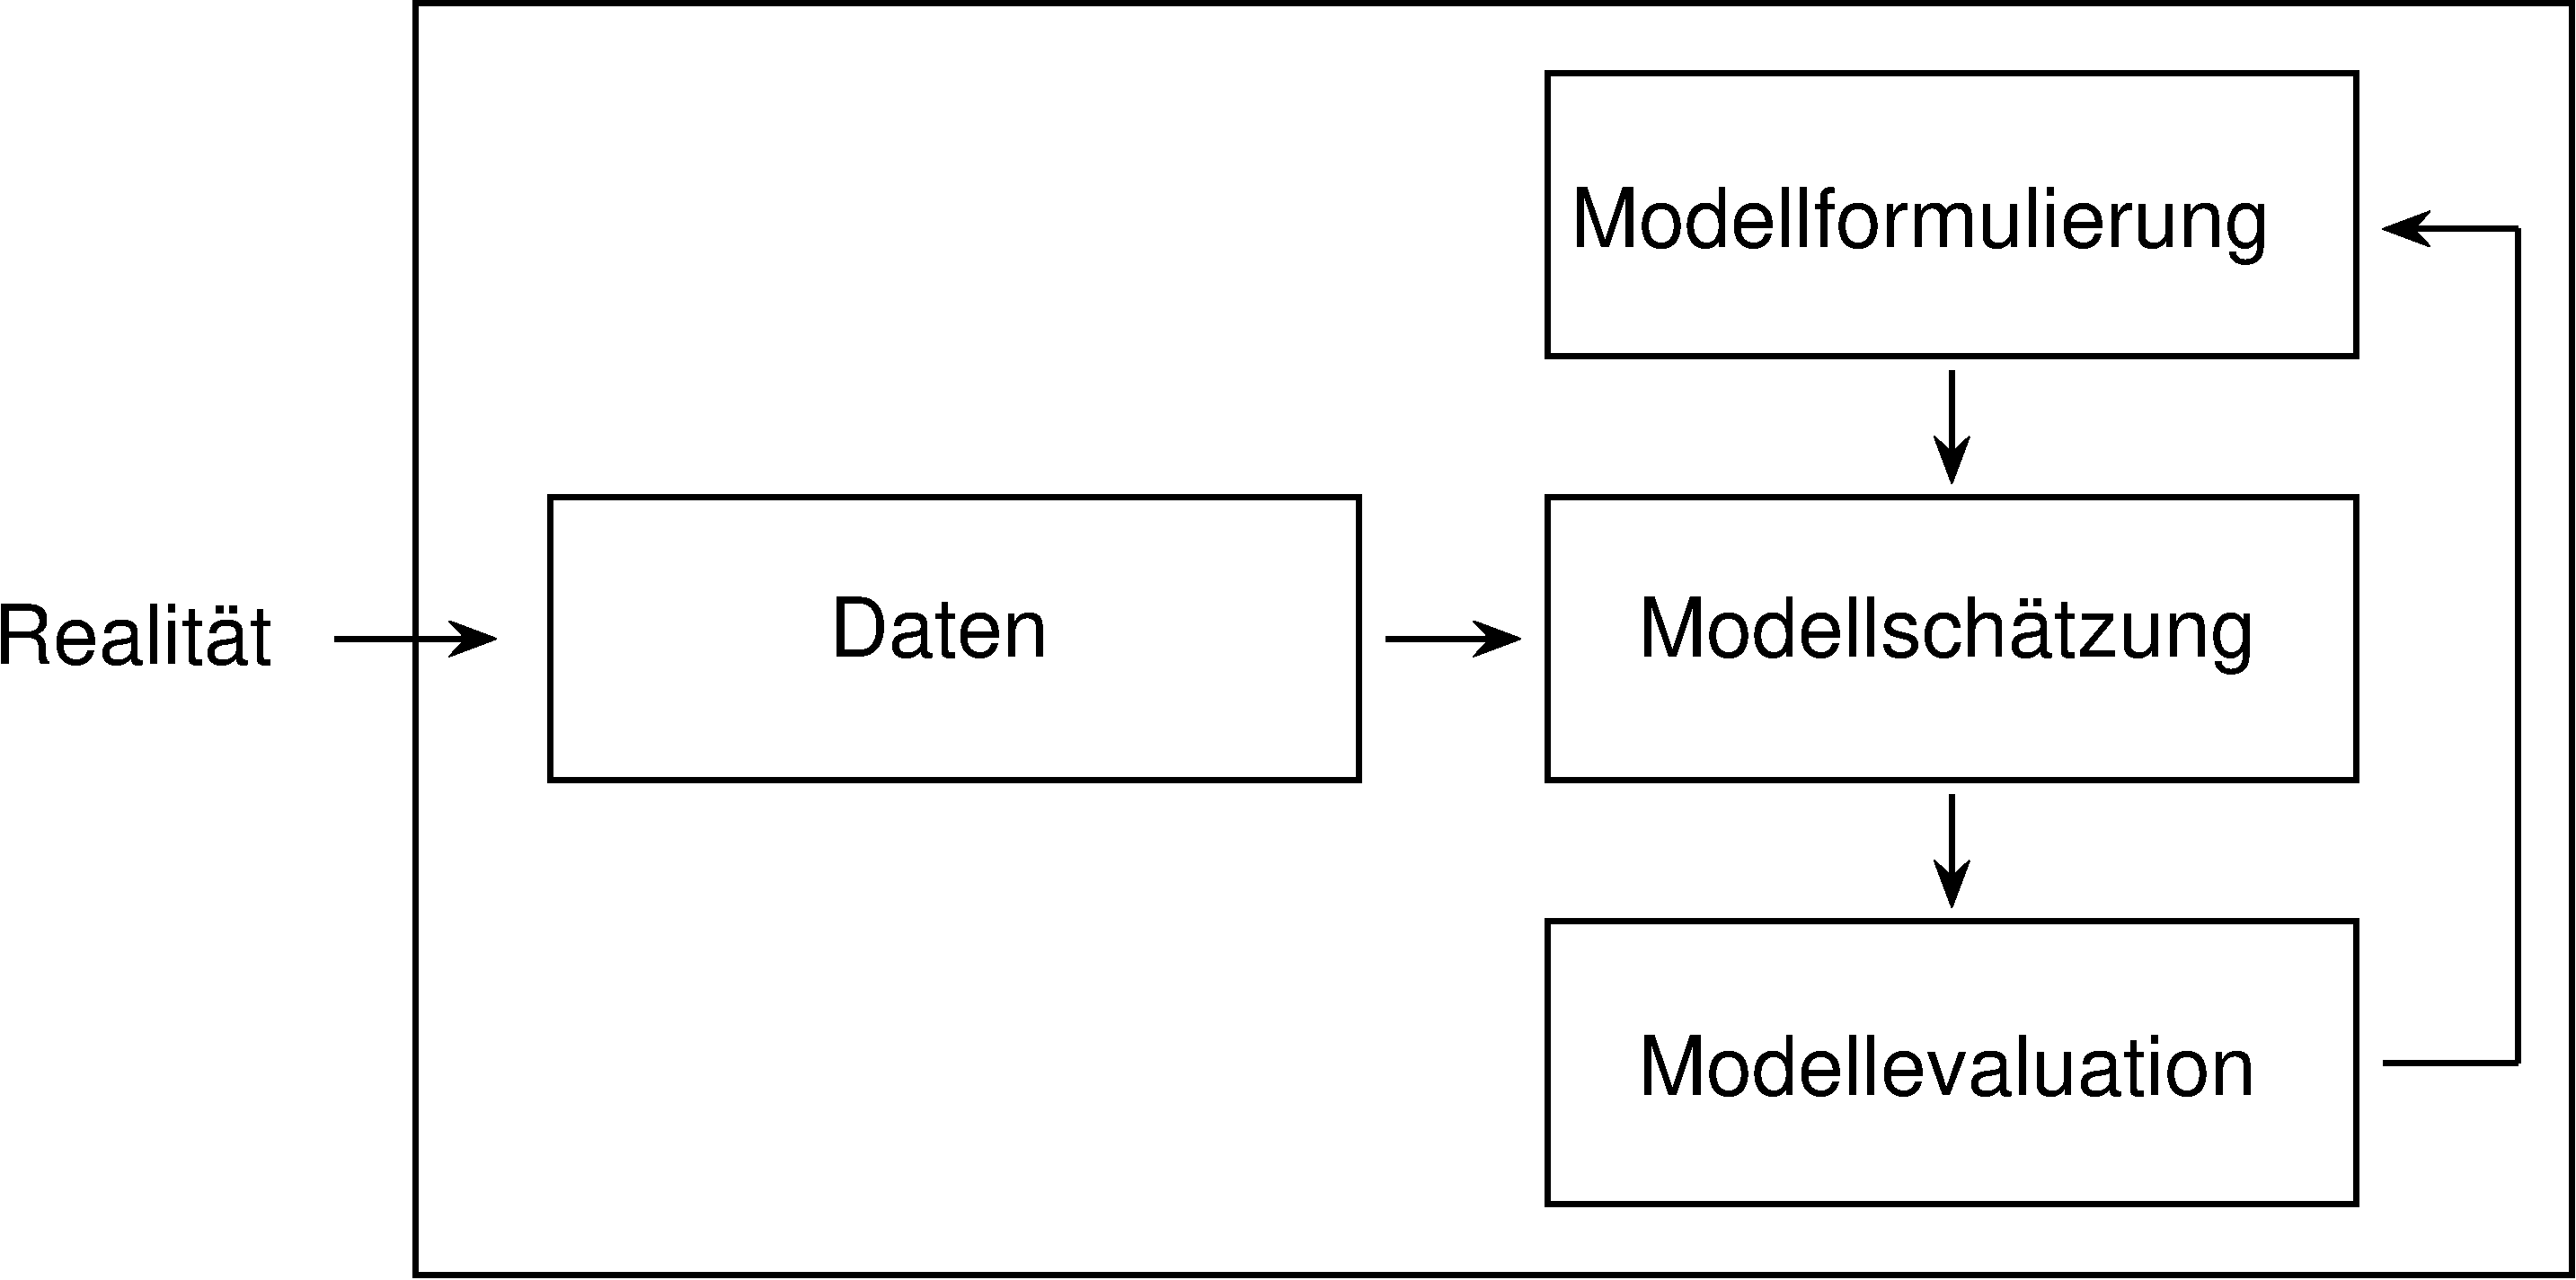
\includegraphics[width=0.9\linewidth]{5_Abbildungen/alm_5_wissenschaft} \end{center}
\end{frame}

\begin{frame}{Überblick}
\protect\hypertarget{uxfcberblick-2}{}
\vspace{1mm}
\normalsize

Modellformulierung \vspace{1mm} \small \begin{equation}
y = X\beta + \varepsilon, \varepsilon \sim N(0_n,\sigma^2I_n)
\end{equation} \vspace{5mm}

\normalsize

Modellschätzung \small \begin{equation}
\hat{\beta} = (X^TX)^{-1} X^Ty,  \hat{\sigma}^2 = \frac{(y - X\hat{\beta})^T(y - X\hat{\beta})}{n-p}
\end{equation} \vspace{4mm}

\normalsize

Modellevaluation \small \begin{equation}
T = \frac{c^T\hat{\beta} - c^T\beta_0}{\sqrt{\hat{\sigma}^2(X^TX)^{-1}c}}, 
F = \frac{(\hat{\varepsilon}_1^T\hat{\varepsilon}_1 - \hat{\varepsilon}^T\hat{\varepsilon})/p_2}{\hat{\varepsilon}^T\hat{\varepsilon}/(n-p)}
\end{equation}
\end{frame}

\begin{frame}{Überblick}
\protect\hypertarget{uxfcberblick-3}{}
Standardprobleme Frequentistischer Inferenz \small

\noindent (1) Parameterschätzung

Ziel der Parameterschätzung ist es, einen möglichst guten Tipp für die
wahren, aber unbekannten, Parameterwerte (oder eine Funktion derer)
abzugeben, typischerweise basierend auf der Beobachtung einer
Datenrealisierung. \vspace{2mm}

\noindent (2) Konfidenzintervalle

Das Ziel der Bestimmung von Konfidenzintervallen ist es, basierend auf
der Verteilung möglicher Parameterschätzwerte eine quantitative Aussage
über die mit dem Schätzwert assoziierte Unsicherheit zu treffen.
\vspace{2mm}

\noindent (3) Hypothesentests

Das Ziel der Auswertung von Hypothesentests ist es, basierend auf der
angenommenen Verteilung der Daten in einer möglichst sinnvollen Form zu
entscheiden, ob ein wahrer, aber unbekannter Parameterwert, sich in
einer von zwei sich gegenseitig ausschließenden Untermengen des
Parameterraumes, welche man als Hypothesen bezeichnet, liegt.
\end{frame}

\begin{frame}{Überblick}
\protect\hypertarget{uxfcberblick-4}{}
\begin{center}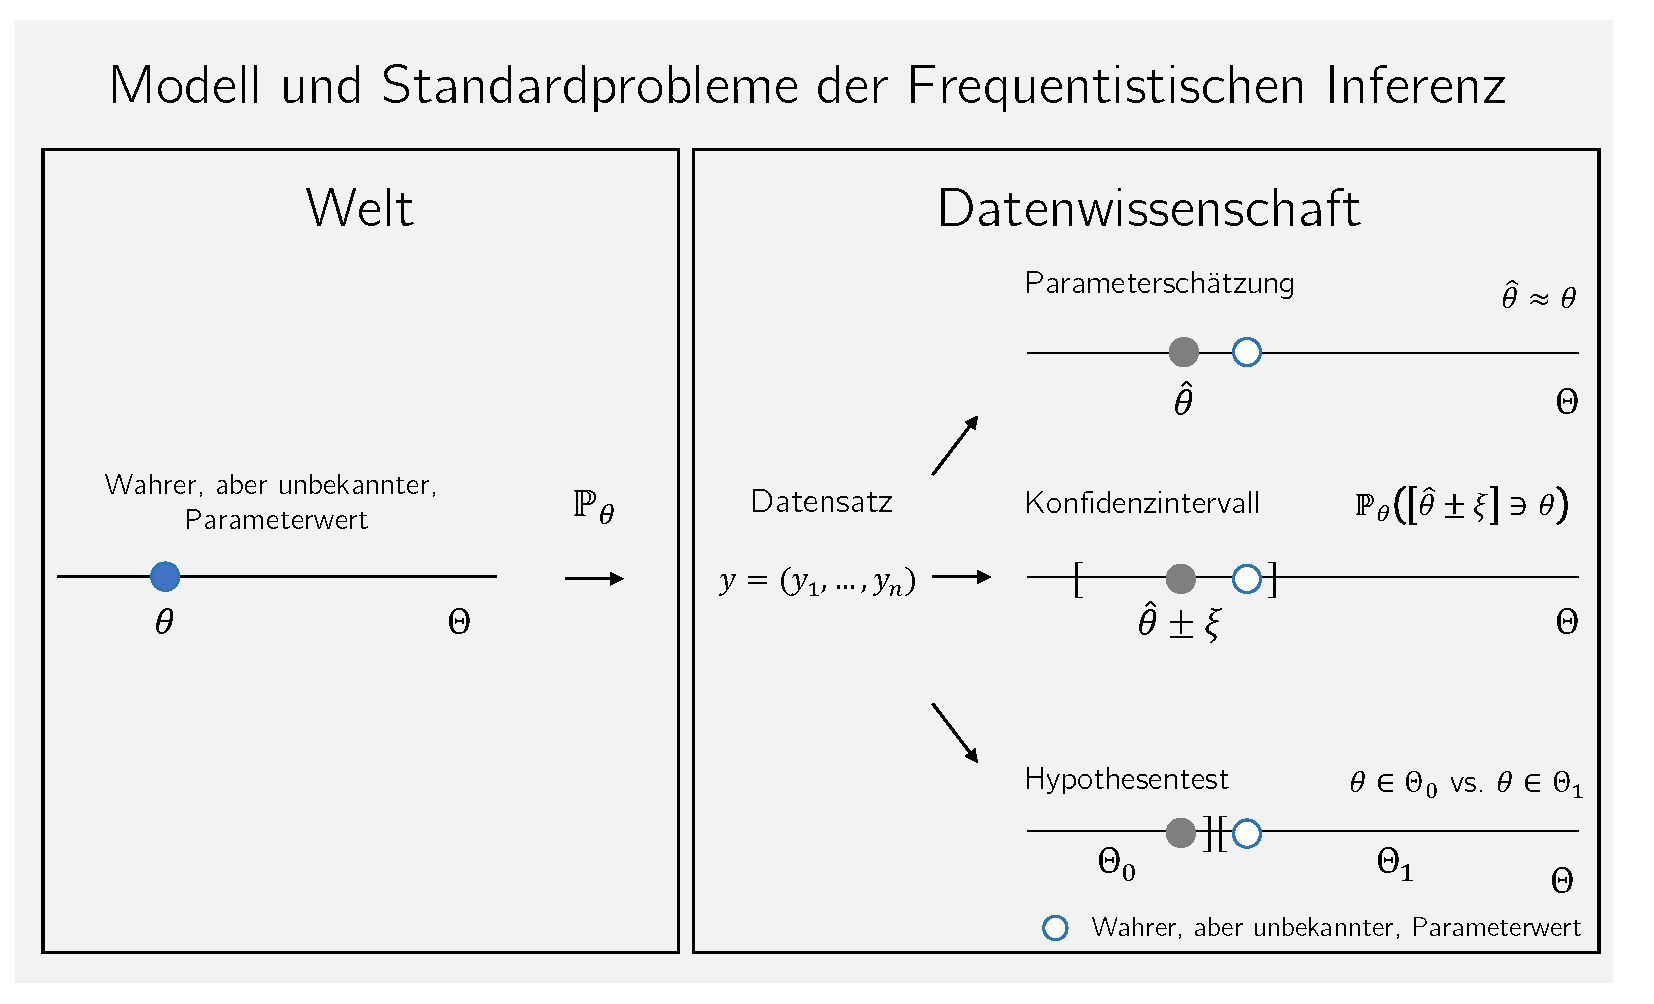
\includegraphics[width=1\linewidth]{5_Abbildungen/alm_5_frequentistische_inferenz} \end{center}
\end{frame}

\begin{frame}{Überblick}
\protect\hypertarget{uxfcberblick-5}{}
\small

Standardannahmen frequentistischer Inferenz

\footnotesize
\setstretch{1.2}

Gegeben sei ein statistisches Modell mit. Es wird angenommen, dass ein
vorliegender Datensatz eine der möglichen Realisierungen der Daten des
Modells ist. Aus frequentistischer Sicht kann man unendlich oft
Datensätze basierend auf einem Modell generieren und zu jedem Datensatz
Schätzer oder Statistiken auswerten, z.B. den Betaparameterschätzer
\vspace{1mm}

\begin{itemize}
\item[] Datensatz (1) : $y^{(1)} = \left(y_1^{(1)}, y_2^{(1)}, ...,y_n^{(1)}\right)^T$  mit $\hat{\beta}^{(1)} = (X^TX)^{-1}X^Ty^{(1)}$
\item[] Datensatz (2) : $y^{(2)} = \left(y_1^{(2)}, y_2^{(2)}, ...,y_n^{(2)}\right)^T$  mit $\hat{\beta}^{(2)} = (X^TX)^{-1}X^Ty^{(2)}$
\item[] Datensatz (3) : $y^{(3)} = \left(y_1^{(3)}, y_2^{(3)}, ...,y_n^{(3)}\right)^T$  mit $\hat{\beta}^{(3)} = (X^TX)^{-1}X^Ty^{(3)}$
\item[] Datensatz (4) : $y^{(4)} = \left(y_1^{(4)}, y_2^{(4)}, ...,y_n^{(4)}\right)^T$  mit $\hat{\beta}^{(4)} = (X^TX)^{-1}X^Ty^{(4)}$
\item[] Datensatz (5) : $y^{(5)} = ...$
\end{itemize}

\vspace{1mm}

Um die Qualität statistischer Methoden zu beurteilen betrachtet die
frequentistische Statistik die Wahrscheinlichkeitsverteilungen von
Schätzern und Statistiken unter Annahme der Datenverteilung. Was zum
Beispiel ist die Verteilung von \(\hat{\beta}^{(1)}\),
\(\hat{\beta}^{(2)}\), \(\hat{\beta}^{(3)}\), \(\hat{\beta}^{(4)}\),
\ldots{} also die Verteilung der Zufallsvariable
\(\hat{\beta} := (X^TX)^{-1}X^Ty\)? Wenn eine statistische Methode im
Sinne der frequentitischen Standardannahmen ``gut'' ist, dann heißt das
also, dass sie bei häufiger Anwendung ``im Mittel gut'' ist. Im
Einzelfall, also im Normalfall nur eines vorliegenden Datensatzes, kann
sie auch ``schlecht'' sein.
\end{frame}

\begin{frame}{Überblick}
\protect\hypertarget{uxfcberblick-6}{}
\setstretch{2}

Anwendungsbeispiele Einheit (5) - (7)

\begin{itemize}
\tightlist
\item
  Unabhängig und identisch normalverteilte Zufallsvariablen \textbar{}
  Einstichproben-T-Test
\item
  Einfache lineare Regression
\end{itemize}

Anwendungsbeispiele Einheit (8) - (13)

\begin{itemize}
\tightlist
\item
  Zweistichproben-T-Tests
\item
  Einfaktorielle Varianzanalyse
\item
  Zweifaktorielle Varianzanalyse
\item
  Multiple Regression
\item
  Kovarianzanalyse
\end{itemize}
\end{frame}

\begin{frame}{}
\protect\hypertarget{section-2}{}
\large
\setstretch{3}
\vfill

Allgemeine Theorie

Unabhängige und identisch normalverteilte Zufallsvariablen

Einfache lineare Regression

Selbstkontrollfragen \vfill
\end{frame}

\begin{frame}{}
\protect\hypertarget{section-3}{}
\large
\setstretch{3}
\vfill

\textbf{Allgemeine Theorie}

Unabhängige und identisch normalverteilte Zufallsvariablen

Einfache lineare Regression

Selbstkontrollfragen \vfill
\end{frame}

\begin{frame}{Allgemeine Theorie}
\protect\hypertarget{allgemeine-theorie}{}
\small
\begin{definition}[Allgemeines Lineares Modell]
\justifying
Es sei
\begin{equation}\label{eq:alm}
y = X\beta + \varepsilon,
\end{equation}
wobei
\begin{itemize}
\item $y$ ein $n$-dimensionaler beobachtbarer Zufallsvektor ist, der \textit{Daten} genannt wird,
\item $X \in \mathbb{R}^{n \times p}$ eine vorgegebene Matrix ist, die \textit{Designmatrix} genannt wird,
\item $\beta \in \mathbb{R}^p$ ein unbekannter Parametervektor ist, der \textit{Betaparametervektor} genannt wird und
\item $\varepsilon$ ein $n$-dimensionaler nicht-beobachtbarer Zufallsvektor ist, der \textit{Zufallsfehler} genannt wird und für den angenommen wird, dass
mit einem unbekannten Varianzparameter $\sigma^2>0$ gilt, dass
\begin{equation}
\varepsilon \sim N\left(0_n, \sigma^2I_n\right).
\end{equation}
\end{itemize}
Dann wird \eqref{eq:alm} \textit{Allgemeines Lineares Modell (ALM) in generativer Form} genannt.
\end{definition}
\end{frame}

\begin{frame}{Allgemeine Theorie}
\protect\hypertarget{allgemeine-theorie-1}{}
\footnotesize

Bemerkungen \setstretch{1.8}

\begin{itemize}
\tightlist
\item
  \justifying \(y\) ist ein Zufallsvektor, weil er aus der Addition des
  Zufallsvektors \(\varepsilon\) zu dem Vektor
  \(X\beta \in \mathbb{R}^n\) resultiert.
\item
  Wir nennen \(X\beta \in \mathbb{R}^n\) den
  \textit{deterministichen Modellaspekt} und \(\varepsilon\) den
  \textit{probabilistischen Modellaspekt}.
\item
  \(n \in \mathbb{N}\) bezeichnet durchgängig die Anzahl an
  Datenpunkten.
\item
  \(p \in \mathbb{N}\) bezeichnet durchgängig die Anzahl an
  Betaparametern.
\item
  Die Gesamtzahl an Parametern des ALMs ist \(p + 1\) (\(p\)
  Betaparameter und \(1\) Varianzparameter).
\item
  Der Betaparametervektor wird auch \textit{Gewichtsvektor} oder
  \textit{Effektvektor} genannt.
\item
  Weil der Kovarianzmatrixparameter von \(\varepsilon\) als sphärisch
  angenommen wird, sind die \(\varepsilon_1,...,\varepsilon_n\)
  unabhängige normalverteilte Zufallsvariablen mit identischem
  Varianzparameter; weil zusätzlich der Erwartungswertparameter von
  \(\varepsilon\) als \(0_n\) angenommen wird, sind die
  \(\varepsilon_1,...,\varepsilon_n\) auch identisch normalverteilte
  Zufallsvariablen.
\item
  Für jede Komponente \(y_i, i = 1,...,n\) von \(y\) impliziert
  \eqref{eq:alm} nach Definition des Matrixprodukts, dass
  \begin{equation}
  y_i = x_{i1}\beta_1 + x_{i2}\beta_2 + \cdots +  x_{ip}\beta_p + \varepsilon_i \mbox{ mit } \varepsilon_i \sim N(0,\sigma^2),
  \end{equation} wobei \(x_{ij} \in \mathbb{R}\) das \(ij\)te Element
  der Designmatrix \(X\) bezeichnet.
\end{itemize}
\end{frame}

\begin{frame}{Allgemeine Theorie}
\protect\hypertarget{allgemeine-theorie-2}{}
\footnotesize
\begin{theorem}[ALM Datenverteilung]
\justifying
\normalfont
Es sei
\begin{equation}
y = X\beta + \varepsilon \mbox{ mit } \varepsilon \sim N(0_n,\sigma^2I_n)
\end{equation}
das ALM in generativer Form. Dann gilt
\begin{equation}
y \sim N(X\beta,\sigma^2I_n).
\end{equation}
\end{theorem}

\underline{Beweis}

Mit dem Theorem zur linear-affinen Transformation multivariater
Normalverteilungen gilt für \(\varepsilon \sim N(0_n,\sigma^2I_n)\) und
\(y := I_n\varepsilon + X\beta\), dass \begin{equation}
y \sim N\left(I_n0_n + X\beta, I_n (\sigma^2 I_n) I_n^T\right) = N(X\beta, \sigma^2 I_n).
\end{equation} Bemerkungen

\begin{itemize}
\tightlist
\item
  Im ALM sind die Daten \(y\) also ein \(n\)-dimensionaler
  normalverteilter Zufallsvektor mit Erwartungswertparameter
  \(X\beta \in \mathbb{R}^n\) und Kovarianzmatrixparameter
  \(\sigma^2I_n \in \mathbb{R}^{n \times n}\).
\item
  Die Komponenten \(y_1,...,y_n\) von \(y\), also die Datenpunkte, sind
  damit unabhängige, aber im Allgemeinen nicht identisch verteilte,
  normalverteilte Zufallsvariablen der Form
  \(y_i \sim N(\mu_i,\sigma^2)\) für \(i = 1,...,n\).
\end{itemize}
\end{frame}

\begin{frame}{}
\protect\hypertarget{section-4}{}
\large
\setstretch{3}
\vfill

Allgemeine Theorie

\textbf{Unabhängige und identisch normalverteilte Zufallsvariablen}

Einfache lineare Regression

Selbstkontrollfragen \vfill
\end{frame}

\begin{frame}{Unabhängige und identisch normalverteilte
Zufallsvariablen}
\protect\hypertarget{unabhuxe4ngige-und-identisch-normalverteilte-zufallsvariablen}{}
\footnotesize

Wir betrachten das Szenario von \(n\) unabhängigen und identisch
normalverteilten Zufallsvariablen mit Erwartungswertparameter
\(\mu \in \mathbb{R}\) und Varianzparameter \(\sigma^2\),
\begin{equation}\label{eq:iid}
y_i \sim N(\mu,\sigma^2) \mbox{ für } i = 1,...,n.
\end{equation} Dann gilt, dass \eqref{eq:iid} äquivalent ist zu
\begin{equation}
y_i = \mu + \varepsilon_i, \varepsilon_i \sim N(0,\sigma^2) \mbox{ für } i = 1,...,n \mbox{ mit unabhängigen } \varepsilon_i.
\end{equation} In Matrixschreibweise ist dies wiederum äquivalent zu
\begin{equation}
y \sim N(X\beta,\sigma^2I_n) \mbox{ mit } X := 1_n\in \mathbb{R}^{n \times 1}, \beta := \mu \in \mathbb{R}^1, \sigma^2>0.
\end{equation}

Bemerkungen

\begin{itemize}
\tightlist
\item
  \justifying Wir kennen dieses Modell bereits aus Einheit (9)
  Grundbegriffe Frequentistischer Inferenz in Wahrscheinlichkeitstheorie
  und Frequentistsche Inferenz, dort haben wir es geschrieben als
  \begin{equation}
  X_1,...,X_n \sim N(\mu,\sigma^2) \mbox{ mit } (\mu,\sigma^2) \in \mathbb{R} \times \mathbb{R}_{>0}.
  \end{equation}
\item
  Bitte verwechseln Sie nicht die Designmatrix
  \(X \in \mathbb{R}^{n \times p}\) des ALMs und die Zufallsvariablen
  \(X_1,...,X_n\) der Szenarien in Wahrscheinlichkeitstheorie und
  Frequentistische Inferenz.
\end{itemize}
\end{frame}

\begin{frame}[fragile]{Unabhängige und identisch normalverteilte
Zufallsvariablen}
\protect\hypertarget{unabhuxe4ngige-und-identisch-normalverteilte-zufallsvariablen-1}{}
\footnotesize

\begin{Shaded}
\begin{Highlighting}[]
\CommentTok{\# Libraries }
\FunctionTok{library}\NormalTok{(MASS)                                }\CommentTok{\# Multivariate Normalverteilung}

\CommentTok{\# Modellformulierung}
\NormalTok{n      }\OtherTok{=} \DecValTok{12}                                  \CommentTok{\# Anzahl von Datenpunkten}
\NormalTok{p      }\OtherTok{=} \DecValTok{1}                                   \CommentTok{\# Anzahl von Betparametern}
\NormalTok{X      }\OtherTok{=} \FunctionTok{matrix}\NormalTok{(}\FunctionTok{rep}\NormalTok{(}\DecValTok{1}\NormalTok{,n), }\AttributeTok{nrow =}\NormalTok{ n)          }\CommentTok{\# Designmatrix}
\NormalTok{I\_n    }\OtherTok{=} \FunctionTok{diag}\NormalTok{(n)                             }\CommentTok{\# n x n Einheitsmatrix}
\NormalTok{beta   }\OtherTok{=} \DecValTok{2}                                   \CommentTok{\# wahrer, aber unbekannter, Betaparameter}
\NormalTok{sigsqr }\OtherTok{=} \DecValTok{1}                                   \CommentTok{\# wahrer, aber unbekannter, Varianzparameter}

\CommentTok{\# Datenrealisierung}
\NormalTok{y      }\OtherTok{=} \FunctionTok{mvrnorm}\NormalTok{(}\DecValTok{1}\NormalTok{, X }\SpecialCharTok{\%*\%}\NormalTok{ beta, sigsqr}\SpecialCharTok{*}\NormalTok{I\_n)  }\CommentTok{\# eine Realisierung eines n{-}dimensionalen ZVs}
\FunctionTok{print}\NormalTok{(y)}
\end{Highlighting}
\end{Shaded}

\begin{verbatim}
>  [1]  2.629  1.446  1.717  1.756  1.753  0.178  3.148  2.622  1.994
> [10] -0.437  2.255  0.600
\end{verbatim}
\end{frame}

\begin{frame}{}
\protect\hypertarget{section-5}{}
\large
\setstretch{3}
\vfill

Allgemeine Theorie

Unabhängige und identisch normalverteilte Zufallsvariablen

\textbf{Einfache lineare Regression}

Selbstkontrollfragen \vfill
\end{frame}

\begin{frame}{Einfache lineare Regression}
\protect\hypertarget{einfache-lineare-regression}{}
\footnotesize

Wir betrachten das generative Modell der einfachen linearen Regression
aus Einheit (1) Regression, \begin{equation}\label{eq:slr}
y_i = \beta_0 + \beta_1x_i + \varepsilon_i, \varepsilon_i \sim N(0,\sigma^2) \mbox{ für } i = 1,...,n,
\end{equation} wobei wir hier nun die Zufallsvariablen \(y_1,...,y_n\)
mit kleinen Buchstaben bezeichnen. \vspace{3mm}

Wir haben bereits gesehen, dass dieses Modell äquivalent ist zu dem
Normalverteilungsmodell der Regession \begin{equation}
y_i \sim N(\mu_i,\sigma^2) \mbox{ mit } \mu_i := \beta_0 + \beta_1x_i \mbox{ für } i = 1,...,n.
\end{equation} \vspace{1mm}

In Matrixschreibweise ist dies wiederrum äquivalent zu \begin{equation}
y \sim N(X\beta,\sigma^2I_n) \mbox{ mit }
X :=
\begin{pmatrix}
1      & x_1        \\
1      & x_2        \\
\vdots & \vdots     \\
1      & x_n
\end{pmatrix}
\in \mathbb{R}^{n \times 2},
\beta :=
\begin{pmatrix}
\beta_0 \\
\beta_1
\end{pmatrix}
\in \mathbb{R}^2,
\sigma^2 > 0.
\end{equation}
\end{frame}

\begin{frame}[fragile]{Einfache lineare Regression}
\protect\hypertarget{einfache-lineare-regression-1}{}
\footnotesize

\begin{Shaded}
\begin{Highlighting}[]
\CommentTok{\# Libraries }
\FunctionTok{library}\NormalTok{(MASS)                                }\CommentTok{\# Multivariate Normalverteilung}

\CommentTok{\# Modellformulierung}
\NormalTok{n      }\OtherTok{=} \DecValTok{10}                                  \CommentTok{\# Anzahl von Datenpunkten}
\NormalTok{p      }\OtherTok{=} \DecValTok{2}                                   \CommentTok{\# Anzahl von Betaparametern}
\NormalTok{x      }\OtherTok{=} \DecValTok{1}\SpecialCharTok{:}\NormalTok{n                                 }\CommentTok{\# Prädiktorwerte}
\NormalTok{X      }\OtherTok{=} \FunctionTok{matrix}\NormalTok{(}\FunctionTok{c}\NormalTok{(}\FunctionTok{rep}\NormalTok{(}\DecValTok{1}\NormalTok{,n),x), }\AttributeTok{nrow =}\NormalTok{ n)     }\CommentTok{\# Designmatrix}
\NormalTok{I\_n    }\OtherTok{=} \FunctionTok{diag}\NormalTok{(n)                             }\CommentTok{\# n x n Einheitsmatrix}
\NormalTok{beta   }\OtherTok{=} \FunctionTok{matrix}\NormalTok{(}\FunctionTok{c}\NormalTok{(}\DecValTok{0}\NormalTok{,}\DecValTok{1}\NormalTok{), }\AttributeTok{nrow =}\NormalTok{ p)            }\CommentTok{\# wahrer, aber unbekannter, Betaparameter}
\NormalTok{sigsqr }\OtherTok{=} \DecValTok{1}                                   \CommentTok{\# wahrer, aber unbekannter, Varianzparameter}

\CommentTok{\# Datenrealisierung}
\NormalTok{y      }\OtherTok{=} \FunctionTok{mvrnorm}\NormalTok{(}\DecValTok{1}\NormalTok{, X }\SpecialCharTok{\%*\%}\NormalTok{ beta, sigsqr}\SpecialCharTok{*}\NormalTok{I\_n)  }\CommentTok{\# eine Realisierung eines n{-}dimensionalen ZVs}
\FunctionTok{print}\NormalTok{(y)}
\end{Highlighting}
\end{Shaded}

\begin{verbatim}
>  [1]  1.36  2.47  2.09  4.54  4.95  5.48  5.14  8.51  7.37 12.07
\end{verbatim}
\end{frame}

\begin{frame}{Einfache lineare Regression}
\protect\hypertarget{einfache-lineare-regression-2}{}
\footnotesize

\vspace{4mm}

\begin{center}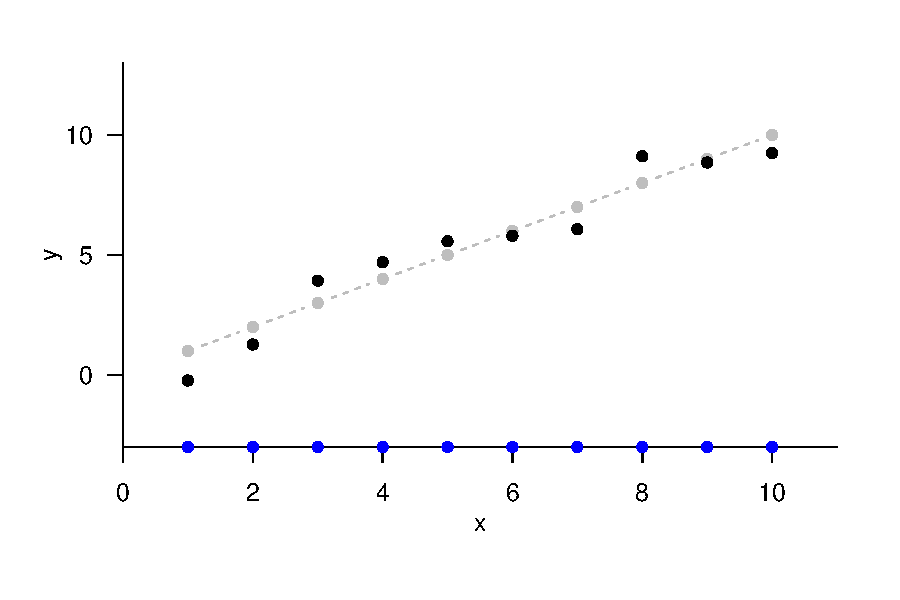
\includegraphics[width=0.85\linewidth]{5_Abbildungen/alm_5_elr} \end{center}
\vspace{-4mm}
\small
\center

\textcolor{blue}{$\bullet$} \(x_i\) \hspace{2mm}
\textcolor{grey}{$\bullet$} \(X\beta\) \mbox{ für } \(\beta_0 := 0\),
\(\beta_1 := 1\) \hspace{2mm} \hspace{2mm} \textcolor{black}{$\bullet$}
\((x_i,y_i)\)
\end{frame}

\begin{frame}{}
\protect\hypertarget{section-6}{}
\large
\setstretch{3}
\vfill

Allgemeine Theorie

Unabhängige und identisch normalverteilte Zufallsvariablen

Einfache lineare Regression

\textbf{Selbstkontrollfragen} \vfill
\end{frame}

\begin{frame}{Selbstkontrollfragen}
\protect\hypertarget{selbstkontrollfragen}{}
\footnotesize
\setstretch{2}

\begin{enumerate}
\tightlist
\item
  \justifying Erläutern Sie das naturwissenschaftliche Paradigma
\item
  Erläutern Sie die Standardprobleme der Frequentistischen Inferenz.
\item
  Setzen Sie das naturwissenschaftliche Paradigma und die
  Frequentistische Inferenz in Beziehung.
\item
  Geben Sie die Definition des ALMs in generativer Form wieder.
\item
  Erläutern Sie die deterministischen und probabilistischen Aspekte des
  ALMs.
\item
  Wieviele Parameter hat das ALM mit sphärischer Kovarianzmatrix?
\item
  Warum sind die Komponenten des ALM Zufallsfehler unabhängig und
  identisch verteilt?
\item
  Geben Sie das Theorem zur ALM Datenverteilung wieder.
\item
  Sind die Komponenten des ALM Datenvektors unabhängig und identisch
  verteilt?
\item
  Schreiben Sie das Szenario \(n\) unabhängig und identisch verteilter
  Zufallsvariablen als ALM in Matrixschreibweise.
\item
  Schreiben Sie das Szenario der einfachen linearen Regression als ALM
  in Matrixschreibweise.
\item
  Generieren Sie 100 Datensätze von 12 unabhängig und identisch
  verteilten Zufallsvariablen.
\item
  Generieren Sie 100 Datensätze von eines einfachen linearen
  Regressionsmodels mit 12 äquidistanten Werten der unabhängigen
  Variable im Intervall \([1,2]\), wobei \(x_1 := 1\) und
  \(x_{12} := 2\) sein sollen.
\end{enumerate}
\end{frame}

\end{document}
